%%
\chapter{Domain modeling and goal definition in EMF and \viatra{}}
%%


\begin{figure}[!ht]
	\begin{center}
		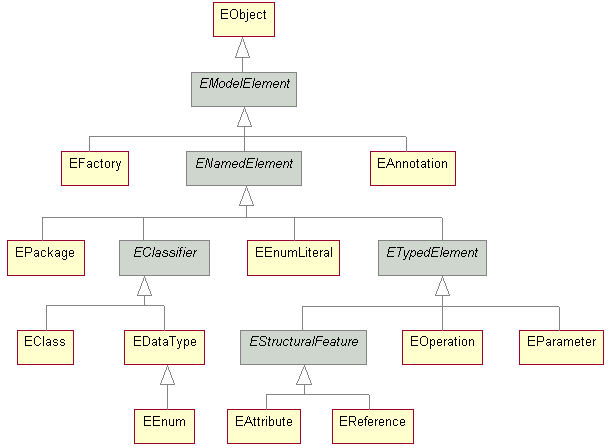
\includegraphics[width=0.5\textwidth]{figures/EcoreHierarchy.png}
		\caption{Hierarchy of Ecore elements}
		\label{fig:ecore-model1}
	\end{center}
\end{figure}

\begin{figure}[!ht]
	\begin{center}
		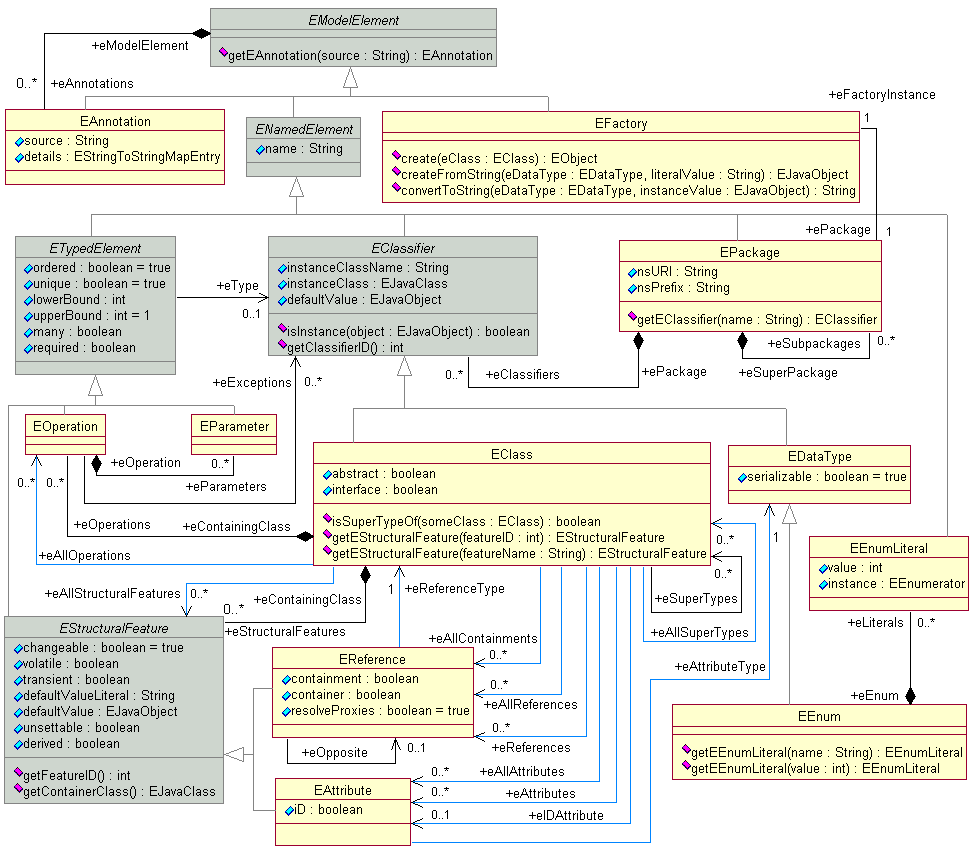
\includegraphics[width=\textwidth]{figures/EcoreRelations.png}
		\caption{Relations between Ecore elements}
		\label{fig:ecore-model2}
	\end{center}
\end{figure}

Domain modeling is an essential part of our framework, as formulating the metamodel of the runtime live model defines the whole process.

In the framework domain modeling are technologically backed up by EMF (Eclipse Modeling Framework) and graph query definition is provided by \viatra{}.

\section{Eclipse Modeling Framework}

\todo{ ecore metamodelling, modelling, EMF api részletezés, stb }

	

\section{\viatra{} query language (VQL)}

As stated before, graph patterns can be defined using \viatra{} query language (VQL). 

\subsection{Pattern definition}
Patterns and its bodies can be given by the \emph{pattern} keyword. 
Parameters must be specified after the parameter name in round brackets. 
Bodies of the pattern are given in curly brackets, separeted by the \emph{or} keyword
\begin{lstlisting}[language = vql]
pattern patternName( p1: Type1, p2: Type2){
	... // Constraints for first body
} or {
	... // Constraints for first body
}
\end{lstlisting}


\subsection{Constraints}
Constraints are given like statements. 
Each constraint is followed by a semicolon.

Type constraint can be given by specifying the type, then the object in round brackets.
\begin{lstlisting}[language = vql][!ht]
pattern patternName( p1 ){
	Type1(p1);
}
\end{lstlisting}

Reference constraint can be given by specifying which type's which reference must be checked, then giving the source and target variables in round brackets.
\begin{lstlisting}[language = vql][!ht]
pattern patternName( p1: Type1, p2: Type2){
Type1.ReferenceLabel(p1, p2);
}
\end{lstlisting}

